\documentclass[10pt]{article}
%\usepackage[a4paper, margin=4cm]{geometry}
\usepackage[spanish,es-tabla]{babel}
\usepackage{natbib}
\usepackage{url}
\usepackage[utf8x]{inputenc}
\usepackage{amsmath}
\usepackage{graphicx}
\usepackage{parskip}
\usepackage{fancyhdr}
\usepackage{vmargin}
\usepackage[ddmmyy]{datetime}
\usepackage{anyfontsize}
\usepackage[table]{xcolor}
\usepackage{pgfplots}
\usepackage{float}
\usepackage{multicol}
\usepackage{siunitx}

\setmarginsrb{2 cm}{1.7 cm}{2 cm}{2 cm}{0 cm}{1 cm}{1 cm}{1.5 cm}


%%%%%%%%%%%%%%%%%%%%%%%%%%%%%%%%%%%%%%%%%%%%%%%%%%%%%%%%%%%%%%%%%%%%%%%%
\begin{document}

    
\begin{center}
    \underline{\textbf{\Large Introducción a los Dispositivos Electrónicos (TB064)}}
    
    \vspace{0.5\baselineskip}
    
    \textbf{\Large Trabajo Práctico Nº2: Transistor TBJ}
    
    \vspace{0.5\baselineskip}
    
    \textbf{\large 1°C 2024} 

    \vspace{0.5\baselineskip}
    
    \textbf{\large Mateo Acosta - 109391} 
\end{center}


%\vspace{1\baselineskip}





%%%%%%%%%%%%%%%%%%%%%%%%%%%%%%%%%%%%%%%%%%%%%%%%%%%%%%%%%%%%%%%%%%%%%%%%%%%%%%%

\section{Obtención de las curvas características}

Se busca hallar las curvas características de un transistor bipolar de juntura PNP.

\textbf{Curva de transferencia}:

\setlength{\columnsep}{2cm} % Establece el espacio entre columnas en 2 cm

\begin{multicols}{2}
    \noindent    
    \begin{figure}[H]
        \centering
        \includegraphics[width=0.8\linewidth]{CircuitoFig_1.png}
        \caption{Circuito para la simulación de la curva de transferencia.}
        \label{fig:circuito1}
    \end{figure}

    \columnbreak
    
    \begin{figure}[H]
        \centering
        \includegraphics[width=0.8\linewidth]{esquemFig1.png}
        \caption{Esquemático para la simulación de la curva de transferencia en \textit{LTspice}}
        \label{fig:circuito1_Spice}
    \end{figure}
\end{multicols}

\setlength{\columnsep}{0.4cm} 
\begin{multicols}{2}
    
    \begin{figure}[H]
        \centering
        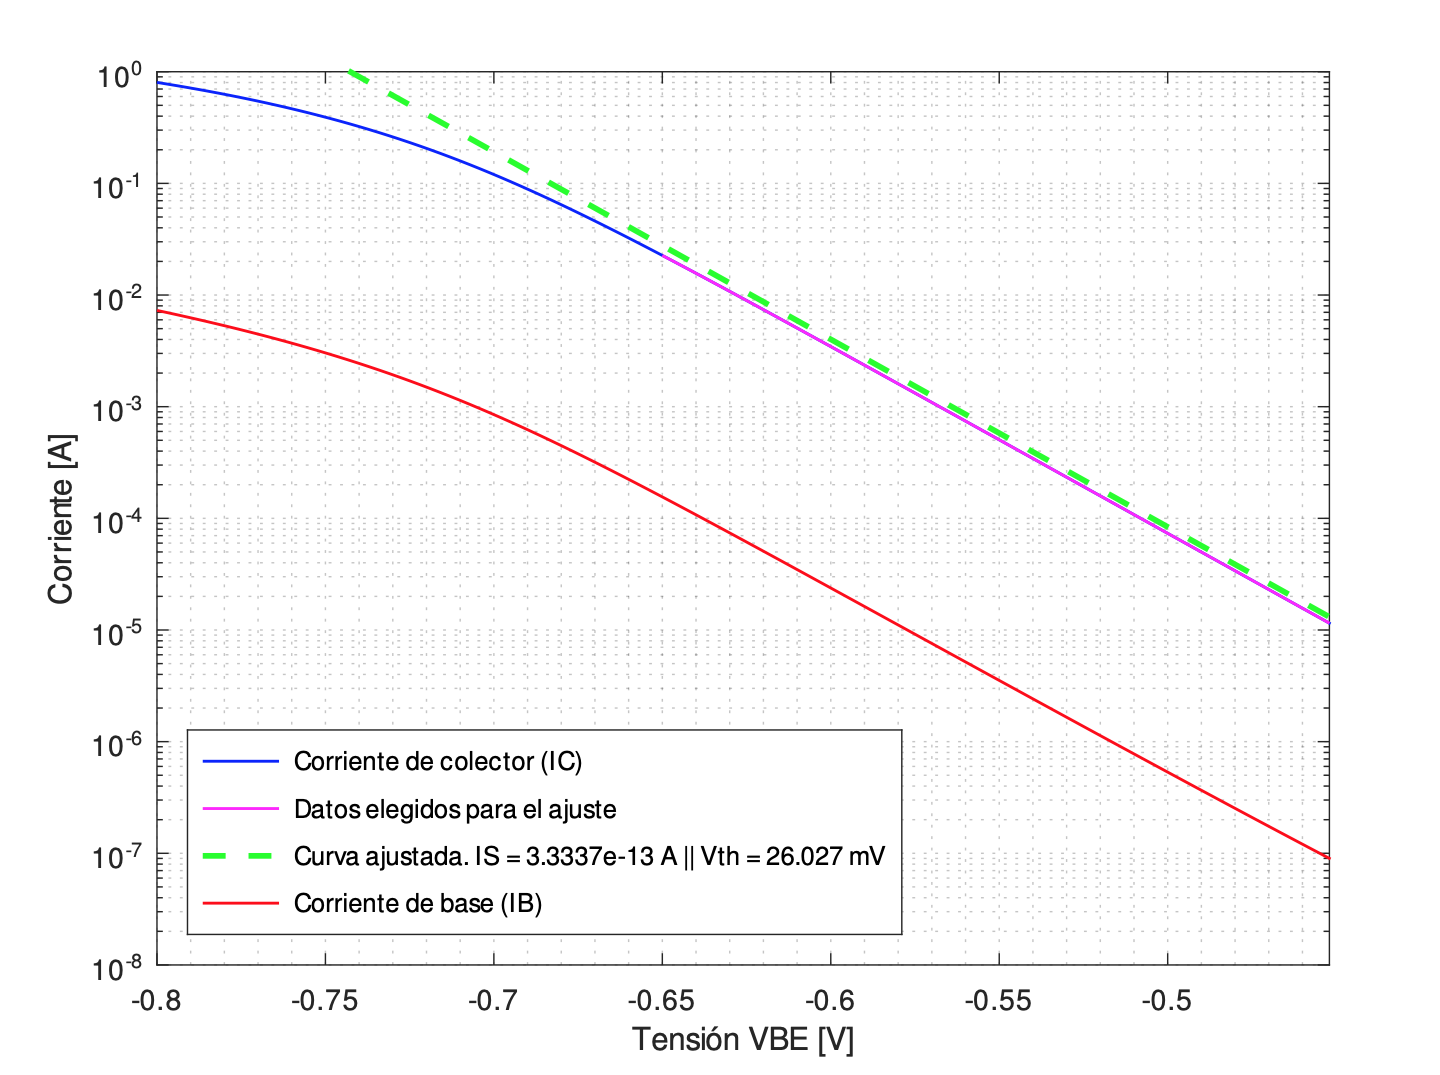
\includegraphics[width=0.95\linewidth]{curvaT.png}
        \caption{Gráfico de la curva de trasferencia simulada}
        \label{fig:curvaTransferencia}
        \end{figure}

    \columnbreak
    
    \noindent
    Se armó el circuito de la Fig. \ref{fig:circuito1} en el software \textit{LTspice}, utilizando un transistor TBJ PNP modelo 2SAR372P5 según el esquemático de la Fig. \ref{fig:circuito1_Spice}. 

    Para la simulación, se mantuvo constate el valor de la fuente $V_{CE} = -3V$ y se realizó un barrido de tensiones entre $-0,8V < V_{BE} < -0,4V$ con un paso de $3mV$. 
    \, A partir de esta simulación se obtuvo una tabla de datos de corriente de base ($I_B$) y corriente de colector ($I_C$) para cada una de las tensiones ($V_{BE}$) aplicadas.

    Tras obtener los valores de ambas corriente, se generó un gráfico en semi-logarítmica (Fig. \ref{fig:curvaTransferencia}) incluyendo el valor absoluto de ambas curvas. 
\end{multicols}

\textbf{Curva de salida}
\setlength{\columnsep}{2cm} % Establece el espacio entre columnas en 2 cm
\begin{multicols}{2}
    \noindent    
    \begin{figure}[H]
        \centering
        \includegraphics[width=0.70\linewidth]{circuitoFig_2.png}
        \caption{Circuito para la simulación de la curva de salida.}
        \label{fig:circuito2}
    \end{figure}

    \columnbreak
    
    \begin{figure}[H]
        \centering
        \includegraphics[width=0.83\linewidth]{esquemFig2.png}
        \caption{Esquemático para la simulación de la curva de salida en \textit{LTspice}}
        \label{fig:circuito2_Spice}
    \end{figure}
\end{multicols}





\setlength{\columnsep}{0.4cm} 

\begin{multicols}{2}
    
    \begin{figure}[H]
        \centering
        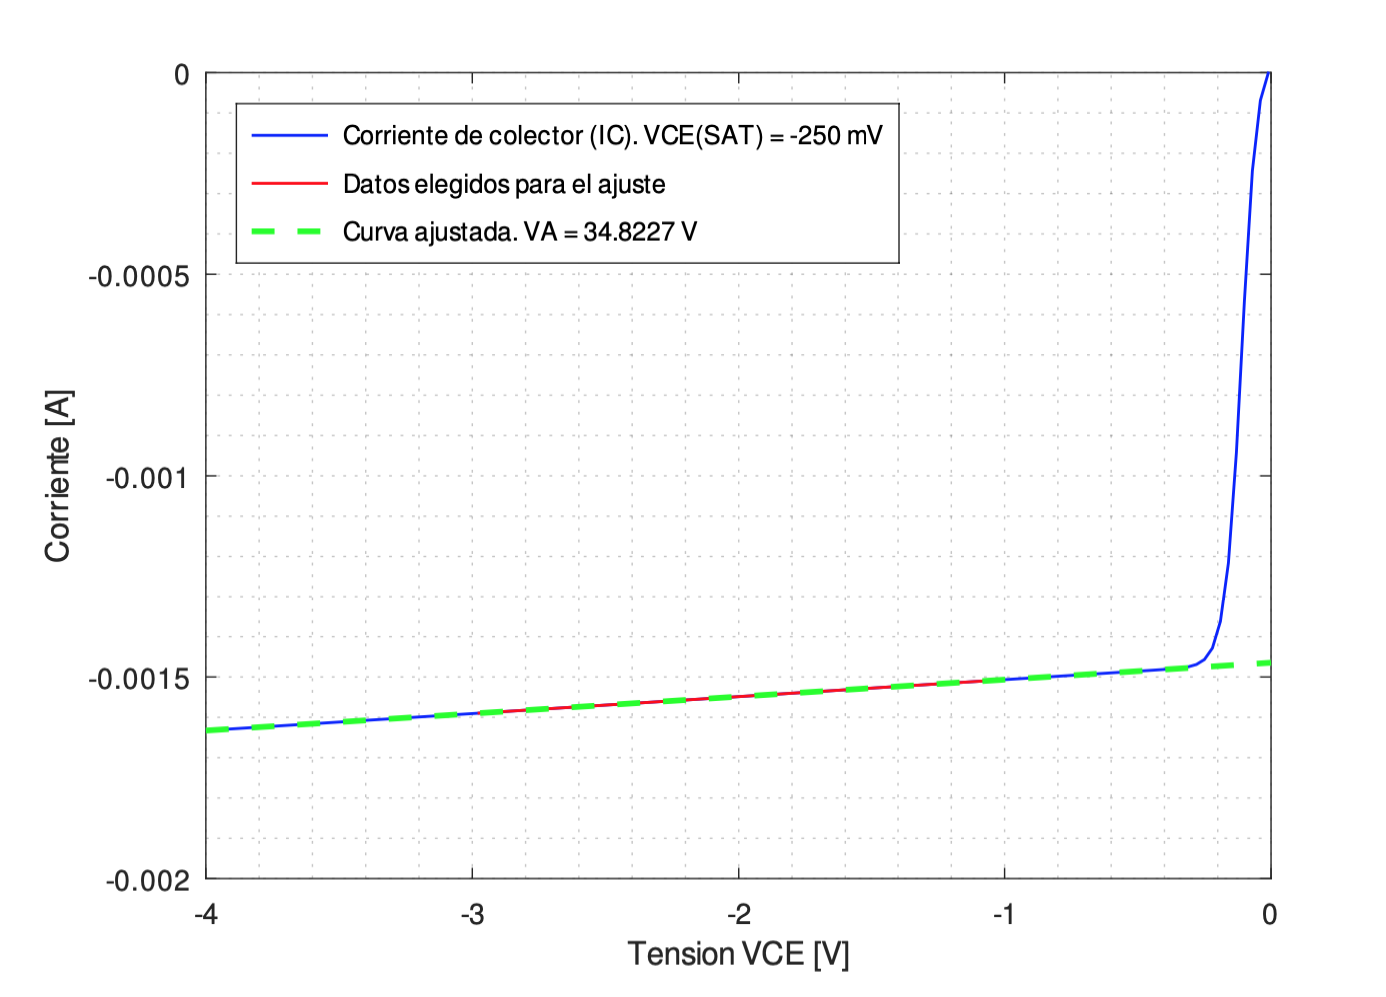
\includegraphics[width=1\linewidth]{curvaS.png}
        \caption{Gráfico de la curva de salida simulada}
        \label{fig:curvaSalida}
        \end{figure}

    \columnbreak
    
    \noindent
    Se armó el circuito de la Fig. \ref{fig:circuito2} en el software \textit{LTspice}, utilizando el mismo transistor TBJ PNP, según el esquemático de la Fig. \ref{fig:circuito2_Spice}. 

    Para la simulación, se utilizó el valor de $I_B = -11\mu A$ para la fuente de corriente de la base, y se realizó un barrido de tensiones entre $-4V < V_{CE} < 0V$ con un paso de $30mV$. 
    
    A partir de esta simulación se obtuvo una tabla de datos de corriente de colector ($I_C$) para cada una de las tensiones ($V_{CE}$) aplicadas.

    Tras obtener los valores se generó un gráfico de la corriente en escala lineal (Fig. \ref{fig:curvaSalida}).
\end{multicols}

%%%%%%%%%%%%%%%%%%%%%%%%%%%%%%%%%%%%%%%%%%%%%%%%%%%%%%%%%%%%%%%%%%%%%%%%%%%%%%
\section{Obtención de parámetros característicos}
Tras realizar los gráficos y sus correspondientes ajustes, se procede a determinar los parámetros característicos del transistor a partir de las diferentes soluciones de la  ec. \ref{ref: ecuacionIC}

\begin{equation}
    I_C = -I_S \cdot  \exp{\left({\frac{V_{BE}}{V_{th}}} \right) \left({1 + \frac{V_{CE}}{V_A}} \right)}  
    \label{ref: ecuacionIC}
\end{equation}

A partir de la curva de transferencia (Fig. \ref{fig:curvaTransferencia}) se seleccionó el rango de tensiones en la región M.A.D del transistor entre $-0,65 < V_{BE} < -0,45$, para realizar el ajuste. Se obtuvo así la recta que mejor se ajusta a la zona en que las corrientes tienden a ser paralelas entre sí. Con esto se pudo calcular la corriente de saturación inversa $I_S$ despreciando el efecto Early.
\begin{equation}
    \ln{|I_C|} = \ln{I_S} \cdot \left( -\frac{1}{V_{th}}\right) \cdot \ln{(-V_{BE})}
\end{equation}

Adicionalmente, se verifica que la diferencia entre la pendiente de la recta ajustada y la inversa de la tensión térmica $V_{th} = 25,8mV$, calculada a una temperatura de trabajo $T = 300 K$, es menor al $1\%$:


\begin{center}
    $V_{th (SIM)} = 26,03\, \mathrm{mV} \qquad \qquad I_S = 333\, \mathrm{fA}$
\end{center}



\begin{multicols}{2}
    
    \begin{figure}[H]
        \centering
        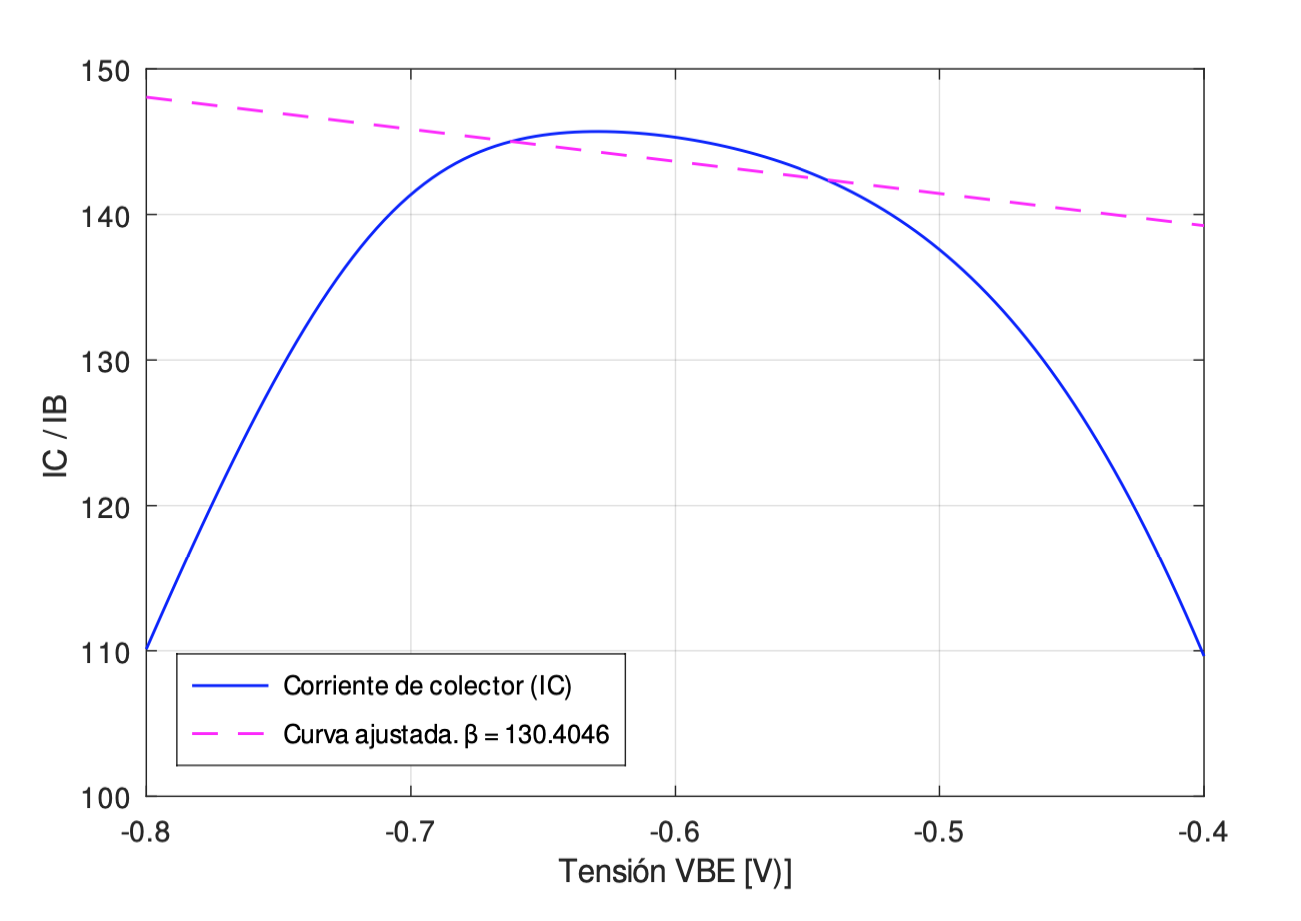
\includegraphics[width=0.9\linewidth]{curvaBeta.png}
        \caption{Gráfico de la curva de salida simulada}
        \label{fig:curvaBeta}
        \end{figure}

    \columnbreak
    
    \noindent
    A partir de la relación entre corriente de base y corriente de colector: $\beta = I_C / I_S$ se determina la ganancia de corriente utilizando el gráfico de la Fig. \ref{fig:curvaBeta} en el cual se selecciono el rango de $-0,65 < V_{BE} < -0,45$ para obtener la recta que mejor se ajusta los puntos en los cuales la relación entre corrientes es mayormente constante.
    
    A esta curva de ajuste se le calculo su ordenada al origen determinando así:
    \begin{equation*}
        \beta = 130,4 
    \end{equation*}
    \vspace{1cm}
\end{multicols}

A partir de la curva de salida (Fig. \ref{fig:curvaSalida}) se obtuvo la recta que mejor ajusta los puntos simulados utilizando el mismo rango de $-0,65 < V_{BE} < -0,45$ de la región M.A.D del transistor. Esta recta se calculó sin tener en cuenta la tensión $V_{BE}$ debido a que la corriente $I_B$ es constante.El corte de esta recta con el eje de las abscisas permitió obtener el valor del parámetro de la tensión de Early: \; $V_A = 36,2 \, \mathrm{V}$


Por inspección visual de la curva de salida se determinó la tensión de saturación en la que se produce el cambio de modo de operación del transistor. Siendo este él punto en el que comienza la separación entre la curva de corriente y la recta de ajuste: \; $V_{CE (SAT)} = -250 \; \mathrm{mV}$

%%%%%%%%%%%%%%%%%%%%%%%%%%%%%%%%%%%%%%%%%%%%%%%%%%%%%%%%%%%%%


\section{Información de los fabricantes}

Los parámetros característicos del transistor se obtuvieron de la hoja de datos: 

ROHM Semiconductor. (2015). 2SAR372P5 PNP -0.7A-120V Middle Power Transistor datasheet (Rev. 001). Mouser Electronics. 



\begin{itemize}
    \item La ganancia de corriente obtenida a partir de la tabla "\textit{Electrical characteristics} $(T_a = 25 ^\circ C)$ "\:se encuentra en el rango de $\beta = (120; 270)$ 

    \item La corriente de saturación inversa $I_S$ no se pudo determinar a partir de las curvas características proporcionadas en la hoja de datos.

    \item La tensión de Early obtenida por un ajuste visual de la curva de salida "\textit{Electrical characteristics curves} $(T_a = 25 ^\circ C). \; Fig(2)$ "\: tiene un valor aproximado de: $V_A = 36,2\; \mathrm{V}$

    \item La tensión de saturación colector-emisor obtenida a partir de la tabla "\textit{Electrical characteristics} $(T_a = 25 ^\circ C)$ "\:se encuentra en el rango de $V_{CE (SAT)} = (-180; -360)\; \mathrm{mV}$ 
\end{itemize}

Se comparan en una tabla los valores obtenidos mediante simulación frente a los del fabricante.

\begin{table}[H]
    \centering
    \begin{tabular}{c|c|c}
         \hline
         Parámetro & Simulación  &  Fabricante\\
         \hline
         $I_S$         &   $333fA$     &          -         \\
         $\beta$       &   $130,4$        &     $120-270$     \\
         $V_{CE(SAT)}$ &   $-250mV$     &     $(-180; -360) mV$     \\
         $V_{A}$       &   $34,8V$     &      $36,2V$    \\
         \hline
    \end{tabular}
    \caption{Comparación de parámetros característicos obtenidos}
    \label{tab:TablaROHMvSpice}
\end{table}

%%%%%%%%%%%%%%%%%%%%%%%%%%%%%%%%%%%%%%%%%%%%%%%%%%%%%%%%%%%%%%%%%%%

\section{Polarización del transistor}

\setlength{\columnsep}{2cm} % Establece el espacio entre columnas en 2 cm

\begin{multicols}{2}
    \noindent    
    \begin{figure}[H]
        \centering
        \includegraphics[width=0.85\linewidth]{CircuitoFig_3.png}
        \caption{Circuito para la polarización del transistor}
        \label{fig:circuito3}
    \end{figure}

    \columnbreak
    
    \begin{figure}[H]
        \centering
        \includegraphics[width=0.95\linewidth]{EsquemaFig3.png}
        \caption{Esquemático para la polarización del transistor en \textit{LTspice}}
        \label{fig:circuito3_Spice}
    \end{figure}
\end{multicols}
Se busca determinar el punto Q del transistor de la Fig . \ref{fig:circuito3} utilizando la leyes de Kirchoff con  $V_{CE_Q} = -3,8V$, $V_{CC} = -5V$, $V_{BE (ON)} = -0,7V$, $I_B = -11\mu A$, $V_A = 34,8 V$ y $\beta = 130,4$: 

\setlength{\columnsep}{0.2cm} 
\begin{multicols}{2}

    \underline{Nodos}:
    \begin{equation*}
        (N_1)\qquad I_{CC} = I_{RB1} + I_C
    \end{equation*}
    \begin{equation*}
        (N_2)\qquad I_{B} + I_{RB2} = I_{RB1}
    \end{equation*}
    \begin{equation*}
        (N_3)\qquad I_{RB2} = I_E + I_{CC}
    \end{equation*}
    
    \columnbreak

    \underline{Mallas}:
    \begin{equation*}
       (I)\qquad V_{CC} - I_C\cdot R_C - V_{CE} = 0
    \end{equation*}
    \begin{equation*}
       (II)\qquad -I_{RB1}\cdot R_{B1} - V_{BC} +I_C\cdot R_C = 0
    \end{equation*}
    \begin{equation*}
       (III)\qquad -I_{RB2}\cdot R_{B2} + V_{BE} = 0
    \end{equation*}
    
\end{multicols}

Para polarizar el transistor en modo activo directo, se adoptó un valor de $R_{B2} = 100k \Omega$. Se desprecia el efecto Early debido a su mínima contribución (menor a $0,1\%$), quedando de esta manera definida la corriente de colector:
\begin{equation}
    I_C = \beta \cdot I_B 
    \label{ref: ecuacionCorrienteColector}
\end{equation}

Una vez hallada la corriente de colector $I_C$ queda definido el punto de polarización:  $Q = (-1,43 mA ;\; -3,8 V)$
\setlength{\columnsep}{0.2cm} 
\begin{multicols}{2}

    \begin{equation*}
    I_C = 130,4 \cdot (-11\mu A) = -1,43mA
    \end{equation*}
    \vspace{0.1cm}
    \begin{equation*}
    R_C = \frac{V_{CC} - V_{CE}}{I_C} = \frac{-5V + 3,8V}{-1,43mA } = 839\: \Omega
    \end{equation*}
    \vspace{0.1cm}
    \begin{equation*}
    I_E = -I_C - I_B = 1,43mA + 11\mu A = 1,44mA
    \end{equation*}
    \vspace{0.1cm}
    \begin{equation*}
    I_{RB2} = \frac{V_{BE}}{R_{B2}} = \frac{0,7V}{100k \Omega} = 7 \mu A
    \end{equation*}

    
    \columnbreak
    \begin{equation*}
    I_{RB1} = I_{B} + I_{RB2} = -11 \mu A + 7 \mu A = -4 \mu A
    \end{equation*}
    \vspace{0.1cm}
    \begin{equation*}
    I_{CC} = I_{RB1} + I_C = -4 \mu A -1,43mA = -1,43 mA
    \end{equation*}
    \vspace{0.1cm}
    \begin{equation*}
    R_{B1} = \frac{V_{CC} + V_{BE}}{I_B -I_{RB2}} = \frac{-5V - 0,7V}{-11\mu A -7 \mu A} = 316k\Omega
    \end{equation*}
    \vspace{0.1cm}
    \begin{equation*}
    V_{BC} = I_C\cdot R_C -I_{RB1}\cdot R_{B1} = 64mV
    \end{equation*}
  
\end{multicols}
*La caída de tensión en cada uno de los resistores se calcula aplicando la ley de Ohm con los valores de tensión y corriente previamente obtenidos. El desarrollo detallado de estos cálculos no se incluye en este informe. 

El circuito analizado se simuló utilizando el esquemático de la Fig. \ref{fig:circuito3_Spice}. Los resultados obtenidos mediante simulación se comparan con los resultados analíticos en una tabla.

\begin{table}[H]
    \centering
    \begin{tabular}{c|c|c|c|c|c}
         Magnitud & $V_{CE}$ & $V_{BE}$  & $I_C$  & $I_B$ & $I_E$ \\
         \hline
         Analítico & $-3,8 V$ & $-0,7V$  & $-1,43mA$ & $-11\mu A$& $1,44 mA$ \\
         Simulación & $-3,9 V$&$-0,6V$&$-1,3mA$&$-8,3\mu A$ & $1,23mA$ \\
         \hline
    \end{tabular}
    \caption{Tabla comparativa entre valores obtenidos analíticamente y por simulación}
    \label{tab:TablaPolarizacion}
\end{table}

Comparando los resultados expuestos en la tabla \ref{tab:TablaPolarizacion}, la diferencia en los valores del punto de polarización es de un $2,6\%$ para la tensión $V_{CE}$ y de un $9.5\%$ para la corriente $I_C$. 
Entre los demás resultados, la mayor diferencia se encuentra en la corriente $I_B$ con un valor de $28\%$. 
%%%%%%%%%%%%%%%%%%%%%%%%%%%%%%%%%%%%%%%%%%%%%%%%%%%%%%%%%%%%%%%%%%%%%%%
\section{Conclusiones}

Al analizar los parámetros característicos obtenidos del transistor, se observó precisión en su cálculo mediante simulación. Los valores obtenidos por este método se encuentran dentro de los rangos aceptados por el fabricante, especificados en la hoja de datos. Con excepción de la corriente de saturación, la cual no pudo ser obtenida a través de las curvas.

En cuanto a la polarización del transistor, si bien se observaron discrepancias entre algunos valores al comparar la simulación con el resultado analítico, la diferencia en el punto de trabajo fue menor al 10\% para ambos valores: tanto para la corriente de colector como para la tensión colector-emisor.


Por estos dos motivos analizados, se puede afirmar que la simulación resulta una herramienta útil al momento trabajar con este modelo particular de transistor, al menos en un rango de tensiones y corrientes similar al analizado en este trabajo.


\end{document}
